%*******************************************************************************
%*********************************** Sixth Chapter *****************************
%*******************************************************************************

\chapter[Phase Measurement Induced Dynamics]
        {Phase Measurement Induced Dynamics\footnote{The results of
            this chapter were first published in
            Ref. \cite{kozlowski2016phase}}}
% Title of the Sixth Chapter

\ifpdf
    \graphicspath{{Chapter6/Figs/Raster/}{Chapter6/Figs/PDF/}{Chapter6/Figs/}}
\else
    \graphicspath{{Chapter6/Figs/Vector/}{Chapter6/Figs/}}
\fi


\section{Introduction}

Light scatters due to its interaction with the dipole moment of the
atoms which for off-resonant light results in an effective coupling
with atomic density, not the matter-wave amplitude. Therefore, it is
challenging to couple light to the phase of the matter-field, as is
typical in quantum optics for optical fields. In the previous chapter
we only considered measurement that couples directly to atomic density
operators just like most of the existing work \cite{LP2009, rogers2014,
  mekhov2012, ashida2015, ashida2015a}. However, we have shown in
section \ref{sec:B} that it is possible to couple to the the relative
phase differences between sites in an optical lattice by illuminating
the bonds between them. Furthermore, we have also shown how it can be
applied to probe the Bose-Hubbard order parameter or even matter-field
quadratures in Chapter \ref{chap:qnd}. This concept has also been
applied to the study of quantum optical potentials formed in a cavity
and shown to lead to a host of interesting quantum phase diagrams
\cite{caballero2015, caballero2015njp, caballero2016,
  caballero2016a}. This is a multi-site generalisation of previous
double-well schemes \cite{cirac1996, castin1997, ruostekoski1997,
  ruostekoski1998, rist2012}, although the physical mechanism is
fundametally different as it involves direct coupling to the
interference terms caused by atoms tunnelling rather than combining
light scattered from different sources.

We have already mentioned that there are three primary avenues in
which the field of quantum optics with ultracold gases can be taken:
nondestructive measurement, quantum measurement backaction, and
quantum optical potentials. All three have been covered in the context
of density-based measurement either here or in other works. However,
coupling to phase observables in lattices has only been proposed and
considered in the context of nondestructive measurements (see Chapter
\ref{chap:qnd}) and quantum optical potentials \cite{caballero2015,
  caballero2015njp, caballero2016, caballero2016a}. In this chapter,
we go in a new direction by considering the effect of measurement
backaction on the atomic gas that results from such coupling.  We
investigate this mechanism using light scattered from these
phase-related observables. The novel combination of measurement
backaction as the physical mechanism driving the dynamics and phase
coherence as the observable to which the optical fields couple to
provides a completely new opportunity to affect and manipulate the
quantum state. We first show how this scheme enables us to prepare
energy eigenstates of the lattice Hamiltonian. Furthermore, in the
second part we also demonstrate a novel type of a projection due to
measurement which occurs even when there is significant competition
with the Hamiltonian dynamics. This projection is fundamentally
different to the standard formulation of the Copenhagen postulate
projection or the quantum Zeno effect \cite{misra1977, facchi2008,
  raimond2010, raimond2012, signoles2014} thus providing an extension
of the measurement postulate to dynamical systems subject to weak
measurement.


\section{Diffraction Maximum and Energy Eigenstates}

In this chapter we will only consider measurement backaction when
$\a_1 = C \hat{B}$ and $\c = \sqrt{2 \kappa} \a_1$ as introduced in
section \ref{sec:B}. We have seen that there are two ways of
engineering the spatial profile of the measurement such that the
density contribution from $\hat{D}$ is suppressed. We will first
consider the case when the profile is uniform, i.e.~the diffraction
maximum of scattered light, when our measurement operator is given by
\begin{equation}
  \B = \Bmax = J^B_\mathrm{max} \sum_j^K \left( \bd_j b_{j+1} b_j
    \bd_{j+1} \right)
  = 2 J^B_\mathrm{max} \sum_k \bd_k b_k \cos(ka),
\end{equation}
where the second equality follows from converting to momentum space,
denoted by index $k$, via
$b_m = \frac{1}{\sqrt{M}} \sum_k e^{-ikma} b_k$ and $b_k$ annihilates
an atom in the Brillouin zone. Note that this operator is diagonal in
momentum space which means that its eigenstates are simply Fock
momentum Fock states. We have also seen in Chapter
\ref{chap:backaction} how the global nature of the jump operators
introduces a nonlocal quadratic term to the Hamiltonian,
$\hat{H} = \hat{H}_0 - i \cd \c / 2$. In order to focus on the
competition between tunnelling and measurement backaction we again
consider non-interacting atoms, $U = 0$. Therefore, $\B$ is
proportional to the Hamiltonian and both operators have the same
eigenstates.

The combined Hamiltonian for the non-interacting gas subject to
measurement of the from $\a_1 = C \B$ is thus
\begin{equation}
  \hat{H} = -J \sum_j \left( \bd_j b_{j+1} + b_j \bd_{j+1} \right) - i
  \gamma \Bmax^\dagger \Bmax.
\end{equation} 
Furthermore, whenever a photon is detected, the operator
$\c = \sqrt{2 \kappa} C \Bmax$ is applied to the wavefunction. We can
rewrite the above equation as
\begin{equation}
  \hat{H} = -\frac{J}{J^B_\mathrm{max}} \Bmax - i \gamma \Bmax^\dagger \Bmax.
\end{equation}
The eigenstates of this operator will be exactly the same as of the
isolated Hamiltonian which we will label as $| h_l \rangle$, where
$h_l$ denotes the corresponding eigenvalue. Therefore, for an initial
state
\begin{equation}
  | \Psi \rangle = \sum_l z_l^0 | h_l \rangle
\end{equation}
it is easy to show that the state after $m$ photocounts and time $t$
is given by
\begin{equation}
  | \Psi (m,t) \rangle = \frac{1}{\sqrt{F(t)}} \sum_l h_l^m z_l^0 e^{[i h_l -
    \gamma(J^B_\mathrm{max}/J)^2 h_l^2]t} | h_l \rangle,
\end{equation}
where $\sqrt{F(t)}$ is the normalisation factor. Therefore, the probability
of being in state $| h_l \rangle$ at time $t$ after $m$ photocounts is
given by
\begin{equation}
  p(h_l, m, t) = \frac{h_l^{2m}} {F(t)} \exp\left[ - 2 \gamma \left(
    \frac{J^B_\mathrm{max}} {J} \right)^2 h_l^2 t \right] |z_l^0|^2.
\end{equation}
As a lot of eigenstates are degenerate, we are actually more
interested in the probability of being in eigenspace with the
eigenvalue $h_l = (J/J^B_\mathrm{max})B_\mathrm{max}$. This probability
is given by
\begin{equation}
  \label{eq:bmax}
  p(B_\mathrm{max}, m, t) = \frac{B_\mathrm{max}^{2m}} {F(t)} \exp\left[ - 2
    \gamma B_\mathrm{max}^2 t \right] p_0 (B_\mathrm{max}),
\end{equation}
where
$p_0(B_\mathrm{max}) = \sum_{J_\mathrm{max} h_l = J B_\mathrm{max}}
|z_l^0|^2$. This distribution will have two distinct peaks at
$B_\mathrm{max} = \pm \sqrt{m/2\kappa |C|^2 t}$ and an initially broad
distribution will narrow down around these two peaks with successive
photocounts. The final state is in a superposition, because we measure
the photon number, $\ad_1 \a_1$ and not field amplitude. Therefore,
the measurement is insensitive to the phase of $\a_1 = C \B$ and we
get a superposition of $\pm B_\mathrm{max}$. This is exactly the same
situation that we saw for the macroscopic oscillations of two distinct
components when the atom number difference between two modes is
measured as seen in Fig. \ref{fig:oscillations}(b). However, this
means that the matter is still entangled with the light as the two
states scatter light with different phase which the photocount
detector cannot distinguish. Fortunately, this is easily mitigated at
the end of the experiment by switching off the probe beam and allowing
the cavity to empty out or by measuring the light phase (quadrature)
to isolate one of the components \cite{mekhov2009pra, mekhov2012,
  atoms2015}.

Unusually, we do not have to worry about the timing of the quantum
jumps, because the measurement operator commutes with the
Hamiltonian. This highlights an important feature of this measurement
- it does not compete with atomic tunnelling, and represents a quantum
non-demolition (QND) measurement of the phase-related observable
\cite{brune1992}. Eq. \eqref{eq:bmax} shows that regardless of the
initial state or the photocount trajectory the system will project
onto a superposition of eigenstates of the $\Bmax$ operator. In fact,
the final state probability distribution would be exactly the same if
we were to simply employ a projective measurement of the same
operator. What is unusual in our case is that this has been achieved
with weak measurement in the presence of significant atomic
dynamics. The conditions for such a measurement have only recently
been rigorously derived in Ref. \cite{weinberg2016} and here we
provide a practical realisation using in ultracold bosonic gases.

This projective behaviour is in contrast to conventional density based
measurements which squeeze the atom number in the illuminated region
and thus are in direct competition with the atom dynamics (which
spreads the atoms), effectively requiring strong couplings for a
projection as seen in the previous chapter. Here a projection is
achieved at any measurement strength which allows for a weaker probe
and thus effectively less heating and a longer experimental
lifetime. Furthermore. This is in contrast to the quantum Zeno effect
which requires a very strong probe to compete effectively with the
Hamiltonian \cite{misra1977, facchi2008, raimond2010, raimond2012,
  signoles2014}. Interestingly, the $\Bmax$ measurement will even
establish phase coherence across the lattice,
$\langle \bd_j b_j \rangle \ne 0$, in contrast to density based
measurements where the opposite is true: Fock states with no
coherences are favoured.

\section{General Model for Weak Measurement Projection}

\subsection{Projections for Incompatible Dynamics and Measurement}

In section \ref{sec:B} we have also shown that it is possible to
achieve a more complicated spatial profile of the
$\B$-measurement. The optical geometry can be adjusted such that each
bond scatters light in anti-phase with its neighbours leading to a
diffraction minimum where the expectation value of the amplitude is
zero. In this case the $\B$ operator is given by
\begin{equation}
  \B = \Bmin = J^B_\mathrm{min} \sum_m^K (-1)^m \hat{B}_m
  = 2 i J^B_\mathrm{min} \sum_k \bd_k b_{k - \pi/a} \sin(ka).
\end{equation}
Note how the measurement operator now couples the momentum mode $k$
with mode $k - \pi/a$. This measurement operator no longer commutes
with the Hamiltonian so it is no longer QND and we do not expect there
to be a steady state as before. In order to understand the measurement
it will be easier to work in a basis in which it is diagonal. We
perform the transformation
$\beta_k = \frac{1}{\sqrt{2}} \left( b_k + i b_{k - \pi/a} \right)$,
$\tilde{\beta}_k = \frac{1}{\sqrt{2}} \left( b_k - i b_{k - \pi/a}
\right)$, which yields the following forms of the measurement operator
and the Hamiltonian:
\begin{equation}
  \label{eq:BminBeta}
  \Bmin = 2 J^B_\mathrm{min} \sum_{\mathrm{RBZ}} \sin(ka) \left( \beta^\dagger_k
    \beta_k - \tilde{\beta}_k^\dagger \tilde{\beta}_k \right),
\end{equation}
\begin{equation}
  \label{eq:H0Beta}
  \hat{H}_0 = - 2 J \sum_{\mathrm{RBZ}} \cos(ka) \left( \beta_k^\dagger
    \tilde{\beta}_k + \tilde{\beta}^\dagger_k \beta_k \right),
\end{equation}
where the summations are performed over the reduced Brilluoin Zone
(RBZ), $0 < k \le \pi/a$, to ensure the transformation is
canonical. We see that the measurement operator now consists of two
types of modes, $\beta_k$ and $\tilde{\beta_k}$, which are
superpositions of two momentum states, $k$ and $k - \pi/a$. Note how a
spatial pattern with a period of two sites leads to a basis with two
modes whilst a uniform pattern had only one mode, $b_k$. Furthermore,
note the similarities to
$\D = \Delta \hat{N} = \hat{N}_\mathrm{even} - \hat{N}_\mathrm{odd}$
which is the density measurement operator obtained by illuminated the
lattice such that neighbouring sites scatter light in anti-phase. This
further highlights the importance of geometry for global measurement.

Trajectory simulations confirm that there is no steady state. However,
unexpectedly, for each trajectory we observe that the dynamics always
ends up confined to some subspace as seen in
Fig. \ref{fig:projections}. In general, this subspace is neither an
eigenspace of the measurement operator or the Hamiltonian. In
Fig. \ref{fig:projections}(b) it in fact clearly consists of multiple
measurement eigenspaces. This clearly distinguishes it from the
fundamental projections predicted by the Copenhagen postulates. It is
also not the quantum Zeno effect which predicts that strong
measurement can confine the evolution of a system as this subspace
must be an eigenspace of the measurement operator \cite{misra1977,
  facchi2008, raimond2010, raimond2012, signoles2014}. Furthermore,
the projection we see in Fig. \ref{fig:projections} occurs for even
weak measurement strengths compared to the Hamiltonian's own
evolution, a regime in which the quantum Zeno effect does not
happen. It is also possible to dissipatively prepare quantum states in
an eigenstate of a Hamiltonian provided it is also a dark state of the
jump operator, $\c | \Psi \rangle = 0$~\cite{diehl2008}. However,
this is also clearly not the case as the final state in
Fig. \ref{fig:projections}(c) is not only not confined to a single
measurement operator eigenspace, it also spans multiple Hamiltonian
eigenspaces. Therefore, the dynamics induced by $\a_1 = C\Bmin$ project
the system into some subspace, but since this does not happen via any
of the mechanisms described above it is not immediately obvious what
this subspace is.

\begin{figure}[hbtp!]
	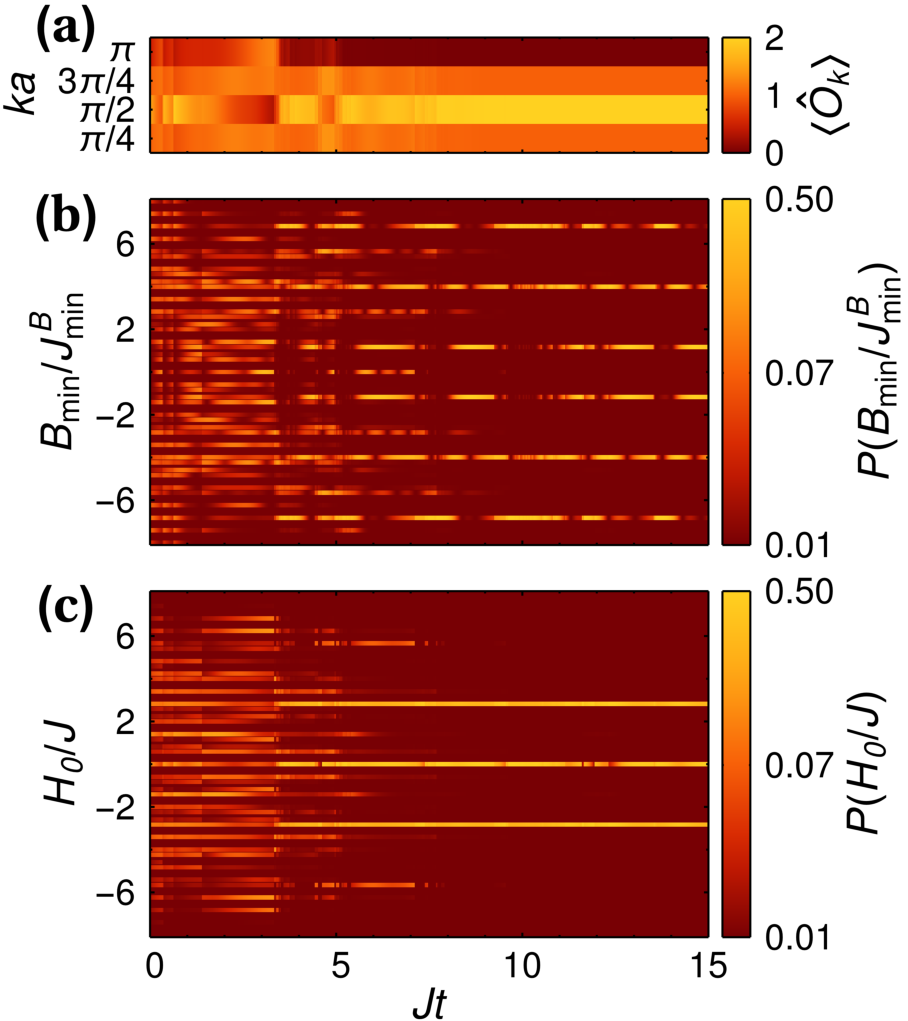
\includegraphics[width=\linewidth]{Projections}
	\caption[Projections for Non-Commuting Observable and
        Hamiltonian] {Subspace projections. Projection to a
          $\mathcal{P}_M$ space for four atoms on eight sites with
          periodic boundary conditions. The parameters used are $J=1$,
          $U=0$, $\gamma = 0.1$, and the initial state was
          $| 0,0,1,1,1,1,0,0 \rangle$. (a) The
          $\langle \hat{O}_k \rangle = \langle \n_k + \n_{k - \pi/a}
          \rangle$ distribution reaches a steady state at
          $Jt \approx 8$ indicating the system has been projected. (b)
          Populations of the $\Bmin$ eigenspaces. (c) Population of
          the $\hat{H}_0$ eigenspaces. Once the projection is achieved
          at $Jt\approx8$ we can see from (b-c) that the system is not
          in an eigenspace of either $\Bmin$ or $\hat{H}_0$, but it
          becomes confined to some subspace. The system has been
          projected onto a subspace, but it is neither that of the
          measurement operator or the
          Hamiltonian. \label{fig:projections}}
\end{figure}

To understand this dynamics we will look at the master equation for
open systems described by the density matrix, $\hat{\rho}$,
\begin{equation}
  \dot{\hat{\rho}} = -i \left[\hat{H}_0, \hat{\rho} \right] + 
  \left[ \c \hat{\rho} \cd - \frac{1}{2} \left( \cd \c \hat{\rho} + \hat{\rho}
      \cd \c \right) \right].
\end{equation}
The following results will not depend on the nature or exact form of
the jump operator $\c$. However, whenever we refer to our simulations
or our model we will be considering $\c = \sqrt{2 \kappa} C(\D + \B)$
as before, but the results are more general and can be applied to ther
setups. This equation describes the state of the system if we discard
all knowledge of the outcome. The commutator describes coherent
dynamics due to the isolated Hamiltonian and the remaining terms are
due to measurement. This is a convenient way to find features of the
dynamics common to every measurement trajectory.

Just like in the preceding chapter we define the projectors of the
measurement eigenspaces, $P_m$, which have no effect on any of the
(possibly degenerate) eigenstates of $\c$ with eigenvalue $c_m$, but
annihilate everything else, thus
$P_m = \sum_{c_n = c_m} | c_n \rangle \langle c_n |,$ where
$| c_n \rangle$ is an eigenstate of $\c$ with eigenvalue $c_n$. Note
that in the specific case of our quantum gas model
$\c = \sqrt{2 \kappa} C(\D + \B)$ so these projectors act on the
matter state. Recall from the previous chapter that this allows us to
decompose the master equation in terms of the measurement basis as a
series of equations $P_m \dot{\hat{\rho}} P_n$. We have seen that for
$m = n$ we obtain decoherence free subspaces,
$P_m \dot{\hat{\rho}} P_m = -i P_m \left[\hat{H}_0, \hat{\rho} \right]
P_m$, where the measurement terms disappear which shows that a state
in a single eigenspace is unaffected by observation. On the other
hand, for $m \ne n$ the Hamiltonian evolution actively competes
against measurement. In general, if $\c$ does not commute with the
Hamiltonian then a projection to a single eigenspace $P_m$ is
impossible unless the measurement is strong enough for the quantum
Zeno effect to occur.

We now go beyond what we previously did and define a new type of
projector 
\begin{equation}
  \mathcal{P}_M = \sum_{m \in M} P_m,
\end{equation}
such that 
\begin{equation}
  \mathcal{P}_M \mathcal{P}_N = \delta_{M,N} \mathcal{P}_M
\end{equation}
\begin{equation}
  \sum_M \mathcal{P}_M = \hat{1}
\end{equation}
where $M$ denotes some arbitrary subspace. The first equation implies that
the subspaces can be built from
$P_m$ whilst the second and third equation are properties of
projectors and specify that these projectors do not overlap and that
they cover the whole Hilbert space. Furthermore, we will also require
that 
\begin{equation}
  [\mathcal{P}_M, \hat{H}_0 ] = 0,
\end{equation}
\begin{equation}
  [\mathcal{P}_M, \c] = 0. 
\end{equation}
The second commutator simply follows from the definition
$\mathcal{P}_M = \sum_{m \in M} P_m$, but the first one is
non-trivial. However, if we can show that
$\mathcal{P}_M = \sum_{m \in M} | h_m \rangle \langle h_m |$, where
$| h_m \rangle$ is an eigenstate of $\hat{H}_0$ then the commutator is
guaranteed to be zero. This is a complex set of requirements and it is
unclear if it is possible to satisfy all of them at once. However, we
note that there exists a trivial case where all these conditions are
satisfied and that is when there is only one such projector
$\mathcal{P}_M = \hat{1}$.

Assuming that it is possible to have non-trivial cases where
$\mathcal{P}_M \ne \hat{1}$ we can write the master equation as
\begin{equation} 
  \label{eq:bigP}
  \mathcal{P}_M \dot{\hat{\rho}} \mathcal{P}_N = -i
  \left[\hat{H}_0, \mathcal{P}_M \hat{\rho} \mathcal{P}_N \right] +
  \left[ \c \mathcal{P}_M \hat{\rho}
  \mathcal{P}_N \cd - \frac{1}{2} \left( \cd \c \mathcal{P}_M \hat{\rho}
  \mathcal{P}_N + \mathcal{P}_M \hat{\rho} \mathcal{P}_N \cd \c \right)
  \right].
\end{equation} 
Crucially, thanks to the commutation relations we were able to divide
the density matrix in such a way that each submatrix's time evolution
depends only on itself. Every submatrix
$\mathcal{P}_M \dot{\hat{\rho}} \mathcal{P}_N$ depends only on the
current state of itself and its evolution is ignorant of anything else
in the total density matrix. This is in contrast to the partitioning
we achieved with $P_m$. Previously we only identitified subspaces that
were decoherence free, i.e.~unaffected by measurement. However, those
submatrices could still couple with the rest of the density matrix via
the coherent term $P_m [\hat{H}_0, \hat{\rho}] P_n$.

We note that when $M = N$ the equations for
$\mathcal{P}_M \hat{\rho} \mathcal{P}_M$ will include decoherence free
subspaces, i.e.~$P_m \hat{\rho} P_m$. Therefore, parts of the
$\mathcal{P}_M \hat{\rho} \mathcal{P}_M$ submatrices will also remain
unaffected by measurement. However, the submatrices
$\mathcal{P}_M \hat{\rho} \mathcal{P}_N$, for which $M \ne N$, are
guaranteed to not contain any of these measurement free subspaces
thanks to the orthogonality of $\mathcal{P}_M$. Therefore, for
$M \ne N$ all elements of $\mathcal{P}_M \hat{\rho} \mathcal{P}_N$
will experience a non-zero measurement term whose effect is always
dissipative/lossy. Furthermore, these coherence submatrices
$\mathcal{P}_M \hat{\rho} \mathcal{P}_N$ are not coupled to any other
part of the density matrix as seen from Eq. \eqref{eq:bigP} and so
they can never increase in magnitude; the remaining coherent evolution
is unable to counteract the dissipative term without an `external
pump' from other parts of the density matrix. The combined effect is
such that all $\mathcal{P}_M \hat{\rho} \mathcal{P}_N$ for which
$M \ne N$ will always go to zero due to dissipation.

When all these cross-terms vanish, we are left with a density matrix
that is a mixed state of the form
$\hat{\rho} = \sum_M \mathcal{P}_M \hat{\rho} \mathcal{P}_M$. Since
there are no coherences, $\mathcal{P}_M \hat{\rho} \mathcal{P}_N$,
this state contains only classical uncertainty about which subspace,
$\mathcal{P}_M$, is occupied - there are no quantum superpositions
between different $\mathcal{P}_M$ spaces. Therefore, in a single
measurement run we are guaranteed to have a state that lies entirely
within a subspace defined by $\mathcal{P}_M$. This is once again
analogous to the qubit example from section \ref{sec:master}.

Such a non-trivial case is indeed possible for our $\hat{H}_0$ and
$\a_1 = C\Bmin$ and we can see the effect in
Fig. \ref{fig:projections}. We can clearly see how a state that was
initially a superposition of a large number of eigenstates of both
operators becomes confined to some small subspace that is neither an
eigenspace of $\a_1$ or $\hat{H}_0$. In this case the projective spaces,
$\mathcal{P}_M$, are defined by the parities (odd or even) of the
combined number of atoms in the $\beta_k$ and $\tilde{\beta}_k$ modes
for different momenta $0 < k < \pi/a$ that are distinguishable to
$\Bmin$. The explanation requires careful consideration of where the
eigenstates of the two operators overlap.

\subsection{Determining the Projection Subspace}

To find $\mathcal{P}_M$ we need to identify the subspaces $M$ which
satisfy the following relation
\begin{equation}
\mathcal{P}_M = \sum_{m \in M} P_m = \sum_{m \in M} | h_m \rangle
\langle h_m |.
\end{equation}
This can be done iteratively by 
\begin{enumerate}
  \item selecting some $P_m$, 
  \item identifying the $| h_m \rangle$ which overlap with this
    subspace,
  \item identifying any other $P_m$ which also overlap with these
    $| h_m \rangle$ from step (ii). 
  \item Repeat 2-3 for all the $P_m$ found in 3 until we
    have identified all the subspaces $P_m$ linked in this way and
    they will form one of our $\mathcal{P}_M$ projectors. If
    $\mathcal{P}_M \ne 1$ then there will be other subspaces $P_m$
    which we have not included so far and thus we repeat this
    procedure on the unused projectors until we identify all
    $\mathcal{P}_M$.
\end{enumerate}
Computationally this can be straightforwardly solved with some basic
algorithm that can compute the connected components of a graph.

The above procedure, whilst mathematically correct and always
guarantees to generate the projectors $\mathcal{P}_M$, is very
unintuitive and gives poor insight into the nature or physical meaning
of $\mathcal{P}_M$. In order to get a better understanding of these
subspaces we need to define a new operator $\hat{O}$, with eigenspace
projectors $R_m$, which commutes with both $\hat{H}_0$ and
$\c$,
\begin{equation}
  [\hat{O}, \hat{H}_0 ] = 0,
\end{equation}
\begin{equation}
  [\hat{O}, \c] = 0. 
\end{equation}
Physically this means that $\hat{O}$ is a compatible observable with
$\c$ and corresponds to a quantity conserved by the Hamiltonian. The
fact that $\hat{O}$ commutes with the Hamiltonian implies that the
projectors can be written as a sum of Hamiltonian eigenstates
\begin{equation}
  R_m = \sum_{h_i = h_m} | h_i \rangle \langle h_i |
\end{equation}
and thus a projector 
\begin{equation}
\mathcal{P}_M = \sum_{m \in M} R_m
\end{equation}
is guaranteed to commute with the Hamiltonian and similarly since
$[\hat{O}, \c] = 0$ $\mathcal{P}_M$ will also commute with $\c$ as
required. Therefore,
\begin{equation}
\mathcal{P}_M = \sum_{m \in M} R_m = \sum_{m \in M} P_m
\end{equation} 
will satisfy all the necessary prerequisites. This is illustrated in
Fig. \ref{fig:spaces}.

\begin{figure}[hbtp!]
	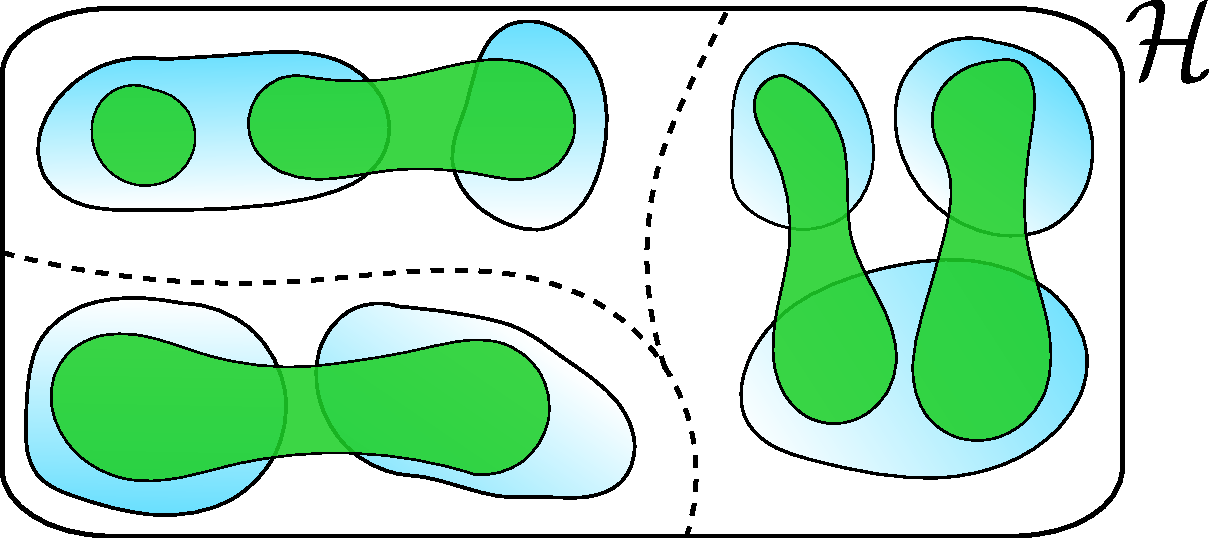
\includegraphics[width=\linewidth]{spaces}
	\caption[A Visual Representation of the Projection Spaces of
        the Measurement]{A visual representation of the projection
          spaces of the measurement. The light blue areas (bottom
          layer) are $R_m$, the eigenspaces of $\hat{O}$. The green
          areas are measurement eigenspaces, $P_m$, and they overlap
          non-trivially with the $R_m$ subspaces. The $\mathcal{P}_M$
          projection space boundary (dashed line) runs through the
          Hilbert space, $\mathcal{H}$, where there is no overlap
          between $P_m$ and $R_m$.  \label{fig:spaces}}
\end{figure}

In the simplest case the projectors $\mathcal{P}_M$ can consist of
only single eigenspaces of $\hat{O}$, $\mathcal{P}_M = R_m$. The
interpretation is straightforward - measurement projects the system
onto a eigenspace of an observable $\hat{O}$ which is a compatible
observable with $\a$ and corresponds to a quantity conserved by the
coherent Hamiltonian evolution. However, this may not be possible and
we have the more general case when
$\mathcal{P}_M = \sum_{m \in M} R_m$. In this case, one can simply
think of all $R_{m \in M}$ as degenerate just like eigenstates of the
measurement operator, $\a$, that are degenerate, can form a single
eigenspace $P_m$. However, these subspaces correspond to different
eigenvalues of $\hat{O}$ distinguishing it from conventional
projections. Instead, the degeneracies are identified by some other
feature.

In our case, it is apparent from the form of $\Bmin$ and $\hat{H}_0$
in Eqs. \eqref{eq:BminBeta} and \eqref{eq:H0Beta} that
\begin{equation}
\hat{O}_k = \beta_k^\dagger \beta_k + \tilde{\beta}_k^\dagger
\tilde{\beta_k} = \n_k + \n_{k - \pi/a}
\end{equation}
commutes with both operators for all $k$. Thus, we can easily
construct 
\begin{equation}
\hat{O} = \sum_\mathrm{RBZ} g_k \hat{O}_k
\end{equation}
for any arbitrary $g_k$. Its eigenspaces, $R_m$, can then be easily
constructed and their relationship with $P_m$ and $\mathcal{P}_M$ is
illustrated in Fig. \ref{fig:spaces} whilst the time evolution of
$\langle \hat{O}_k \rangle$ for a sample trajectory is shown in
Fig. \ref{fig:projections}(a). Note that unlike the $\c$ or $\H_0$ we
can actually see that this observable's distribution does indeed
freeze. These eigenspaces are composed of Fock states in momentum
space that have the same number of atoms within each pair of $k$ and
$k - \pi/a$ modes.

Having identified and appropriate $\hat{O}$ operator we proceed to
identifying $\mathcal{P}_M$ subspaces for the operator
$\Bmin$. Firstly, since $\Bmin$ contains $\sin(ka)$ coefficients atoms
in different $k$ modes that have the same $\sin(ka)$ value are
indistinguishable to the measurement and will lie in the same $P_m$
eigenspaces. This will happen for the pairs ($k$, $\pi/a -
k$). Therefore, the $R_m$ spaces that have the same
$\hat{O}_k + \hat{O}_{\pi/a - k}$ eigenvalues must belong to the same
$\mathcal{P}_M$.

Secondly, if we re-write $\hat{O}$ in terms of the $\beta_k$ and
$\tilde{\beta}_k$ modes we get
\begin{equation} 
  \hat{O} = \sum_{\mathrm{RBZ}} g_k \left(
    \beta^\dagger_k \beta_k + \tilde{\beta}_k^\dagger \tilde{\beta}_k
  \right),
\end{equation}
and so it's not hard to see that
$\B_{\mathrm{min},k} = (\beta^\dagger_k \beta_k -
\tilde{\beta}_k^\dagger \tilde{\beta}_k)$ can have the same
eigenvalues for different values of
$\hat{O}_k = \beta^\dagger_k \beta_k + \tilde{\beta}_k^\dagger
\tilde{\beta}_k$. Specifically, if a given subspace $R_m$ corresponds
to the eigenvalue $O_k$ of $\hat{O}_k$ then the possible values of
$B_{\mathrm{min},k}$ will be $\{-O_k, -O_k + 2, ..., O_k - 2, O_k\}$
just like $\Delta N = N_\mathrm{even} - N_\mathrm{odd}$ can have
multiple possible values for a fixed
$N = N_\mathrm{even} + N_\mathrm{odd}$. Therefore, we can see that all
$R_m$ with even values of $O_k$ will share $B_{\mathrm{min},k}$
eigenvalues and thus they will overlap with the same $P_m$
subspaces. The same is true for odd values of $O_k$. However, $R_m$
with an even value of $O_k$ will never have the same value of
$B_{\mathrm{min},k}$ as a subspace with an odd value of
$O_k$. Therefore, a single $\mathcal{P}_M$ will contain all $R_m$ that
have the same parities of $O_k$ for all $k$, e.g.~if it includes the
$R_m$ with $O_k = 6$, it will also include the $R_m$ for which
$O_k = 0, 2, 4, 6, ..., N$, but not any of $O_k = 1, 3, 5, 7, ..., N$,
where $N$ is the total number of atoms.

Finally, the $k = \pi/a$ mode is special, because $\sin(\pi) = 0$
which means that $B_{\mathrm{min},k=\pi/a} = 0$ always. This in turn
implies that all possible values of $O_{\pi/a}$ are degenerate to the
measurement. Therefore, we exclude this mode when matching the
parities of the other modes.

To illustrate the above let us consider a specific example. Let us
consider two atoms, $N=2$, on eight sites $M=8$. This particular
configuration has eight momentum modes
$ka = \{-\frac{3\pi}{4}, -\frac{\pi}{2}, -\frac{\pi}{4}, 0,
\frac{\pi}{4}, \frac{\pi}{2}, \frac{3\pi}{4}, \pi\}$ and so the RBZ
has only four modes,
$\mathrm{RBZ} := \{\frac{\pi}{4}, \frac{\pi}{2}, \frac{3\pi}{4},
\pi\}$. There are 10 different ways of splitting two atoms into these
four modes and thus we have 10 different
$R_m = \{O_{\pi/4a}, O_{\pi/2a} ,O_{3\pi/4a} ,O_{\pi/a}\}$ eigenspaces
of $\hat{O}$
\begin{table}[!htbp]
  \centering
  \begin{tabular}{l c c}
    \toprule
    $m$ & $R_m$ & Possible values of $B_\mathrm{min}$ \\ \midrule
    0 & $\{2,0,0,0\}$ & $ -\sqrt{2}, 0, \sqrt{2}  $ \\
    1 & $\{1,1,0,0\}$ & $  -\frac{1 + \sqrt{2}}{\sqrt{2}}, -\frac{1
                        - \sqrt{2}}{\sqrt{2}}, \frac{1
                        - \sqrt{2}}{\sqrt{2}}, \frac{1 +
                        \sqrt{2}}{\sqrt{2}}  $ \\ 
    2 & $\{1,0,1,0\}$ & $  -\sqrt{2}, 0, \sqrt{2}  $ \\
    3 & $\{1,0,0,1\}$ & $  -\frac{1}{\sqrt{2}},
                        \frac{1}{\sqrt{2}}  $ \\
    4 & $\{0,2,0,0\}$ & $  -2, 0, 2  $ \\
    5 & $\{0,1,1,0\}$ & $  -\frac{1 + \sqrt{2}}{\sqrt{2}}, -\frac{1
                        - \sqrt{2}}{\sqrt{2}}, \frac{1
                        - \sqrt{2}}{\sqrt{2}}, \frac{1 +
                        \sqrt{2}}{\sqrt{2}} $ \\
    6 & $\{0,1,0,1\}$ & $  -1, 1  $ \\
    7 & $\{0,0,2,0\}$ & $  -\sqrt{2}, 0, \sqrt{2}  $ \\
    8 & $\{0,0,1,1\}$ & $  -\frac{1}{\sqrt{2}},
                        \frac{1}{\sqrt{2}}  $ \\
    9 & $\{0,0,0,2\}$ & $0$ \\
    \bottomrule
  \end{tabular}
  \caption[Eigenspace Overlaps]{A list of all $R_m$ eigenspaces for $N
    = 2$ atoms at $M = 8$ sites. The third column displays the eigenvalues of
    all the eigenstates of $\Bmin$ that lie in the given $R_m$.}
  \label{tab:Rm}
\end{table}
In the third column we have also listed the eigenvalues of the $\Bmin$
eigenstates that lie within the given $R_m$.

We note that $ka = \pi/4$ will be degenerate with $ka = 3\pi/4$ since
$\sin(ka)$ is the same for both. Therefore, we already know that we
can combine $(R_0, R_2, R_7)$, $(R_1, R_5)$, and $(R_3, R_8)$, because
those combinations have the same $O_{\pi/4a} + O_{3\pi/4a}$
values. This is very clear in the table as these subspaces span
exactly the same values of $B_\mathrm{min}$, i.e.~the have exactly the
same values in the third column.

Now we have to match the parities. Subspaces that have the same parity
combination for the pair $(O_{\pi/4a} + O_{3\pi/4a}, O_{\pi/2a})$ will
be degenerate in $\mathcal{P}_M$. Note that we excluded $O_{\pi/a}$,
because as we discussed earlier they are all degenerate due to
$\sin(\pi) = 0$. Therefore, the (even,even) subspace will include
$(R_0, R_2, R_4, R_7, R_9)$, the (odd,even) will contain $(R_3, R_8)$,
the (even, odd) will contain $(R_6)$ only, and the (odd, odd) contains
$(R_1, R_5)$. These overlaps should be evident from the table as we
can see that these combinations combine all $R_m$ that share any
eigenstates of $\Bmin$ with the same eigenvalues.

Therefore, we have ended up with four distinct $\mathcal{P}_M$ subspaces
\begin{align}
\mathcal{P}_\mathrm{even,even} = & R_0 + R_2 + R_4 + R_7 + R_9
  \nonumber \\
\mathcal{P}_\mathrm{odd,even} = & R_3 + R_8 \nonumber \\
\mathcal{P}_\mathrm{even,odd} = & R_6 \nonumber \\
\mathcal{P}_\mathrm{odd,odd} = & R_1 + R_5 \nonumber.
\end{align}
At this point it should be clear that these projectors satisfy all our
requirement. The conditions $\sum_M \mathcal{P}_M = 1$ and
$\mathcal{P}_M \mathcal{P}_N = \delta_{M,N} \mathcal{P}_M$ should be
evident from the form above. The commutator requirements are also
easily satisfied since the subspaces $R_m$ are of an operator that
commutes with both the Hamiltonian and the measurement operator. And
finally, one can also verify using the table that all of these
projectors are built from complete subspaces of $\Bmin$ (i.e.~each
subspace $P_m$ belongs to only one $\mathcal{P}_M$) and thus
$\mathcal{P}_M = \sum_{m \in M} P_m$.

\section{Conclusions}

In summary we have investigated measurement backaction resulting from
coupling light to an ultracold gas's phase-related observables. We
demonstrated how this can be used to prepare the Hamiltonian
eigenstates even if significant tunnelling is occuring as the
measurement can be engineered to not compete with the system's
dynamics. Furthermore, we have shown that when the observable of the
phase-related quantities does not commute with the Hamiltonian we
still project to a specific subspace of the system that is neither an
eigenspace of the Hamiltonian or the measurement operator. This is in
contrast to quantum Zeno dynamics \cite{misra1977, facchi2008,
  raimond2010, raimond2012, signoles2014} or dissipative state
preparation \cite{diehl2008}. We showed how this projection is
essentially an extension of the measurement postulate to weak
measurement on dynamical systems where the competition between the two
processes is significant.
